\chapter{Feature Extraction}\label{final}
\section{Maximal Points}
First all the points with local maxima are extracted, the points which are greater than its previous and next value. Then the points with value less than a threshold value is discarded. The threshold value is obtained from the equation[…….], where u is mean, sd is standard deviation and k is the whole number value set by the user. The value of k is found out by trial and error method, and depends from user to user.

\section{Gait Cycle Points} 
The remaining points forms the gait cycle. cycle is sometimes called the walking cycle. It exists  between any two consecutive heel strike of the same leg\cite{oregonstate}.

\begin{figure}
\center{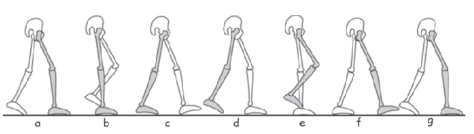
\includegraphics[scale=0.43]{pictures/gaitcycle.png}}\cite{oregonstate}
\caption{Single Gait Cycle.}
\end{figure}

\subsection{Average Gait Cycle} 
Average Gait Cycle(AGC)\cite{oregonstate} is defined as shown in the following equation.\\

$\begin{displaystyle}
  AGC = \left.
  \begin{cases}
    gaitcycle_k \ | & d_k = argmin(\frac{1}{N}\sum_{j=1}^{N} dtw(gaitcycle_k,gaitcycle_j))
  \end{cases}
  \right\} 
\end{displaystyle}$ \cite{oregonstate}
\newline
The term average could be misleading here as we are not taking average of all gait cycles,instead we compare each gait cycle with every other gait cycle and the one which has maximum resemblance to other gait cycles is considered as the average gait cycle.

It has an advantage, every extracted gait cycle may not be a gait cycle in reality instead it can be noise. Hence those noisy gait cycle will least resemble to other gait cycle and could not be an average gait cycle. 

Had we been taken the average of all gait cycle the noisy gait cycle would have been considered distorting average gait cycle.

\begin{figure}
\center{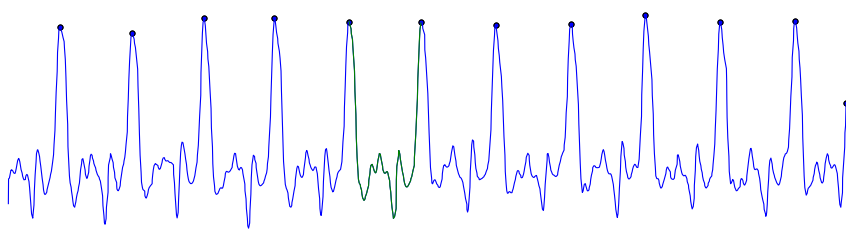
\includegraphics[scale=0.4]{pictures/agc_left_crop.png}}
\caption{AGC of left leg(in black).}
\end{figure}

\begin{figure}
\center{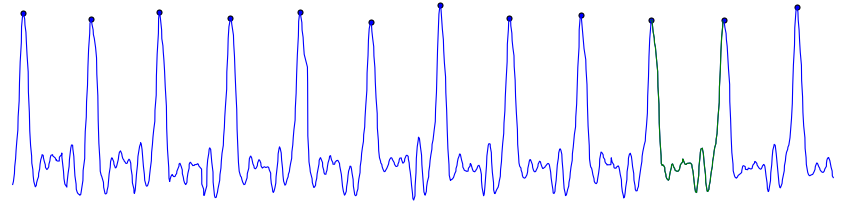
\includegraphics[scale=0.4]{pictures/agc_right_crop.png}}
\caption{AGC of right leg(in black).}
\end{figure}


\section{Dynamic Time Wrapping}
The time domain technique that we used to compare any two gait cycle is Dynamic Time Wrapping(DTW)\cite{dtw1}. DTW is a pattern matching technique. We don’t have to normalize the length/duration of each gait cycle taking advantage of the property of DTW.


\begin{verbatim}

    dwt(array x,array y){
        cost[0][0] := d(x[0], y[0]);
        for i from 1 to nRows-1 
            cost[i][0] := cost[i-1][0] + d(x[i], y[0]);
        for i from 1 to nCols-1
            cost[0][i] := cost[0][i-1] + d(x[0], y[i]);
        for i from 1 to nRows-1
            for j from 1 to nCols-1{
                mm := min( cost[i][j-1], cost[i-1][j-1] ) ;
                cost[i][j] := min( cost[i-1][j], mm ) + d(x[i], y[j]);
            }
        return cost[nRows-1][nCols-1];
    }
    WHERE d(x, y) = | x - y |
\end{verbatim} \cite{dtw1}
% Where \begin{verbatim}\end{verbatim}\cite{dtw1}
